\section{Arquitectura}

	\begin{figure}[H]
			\centering
			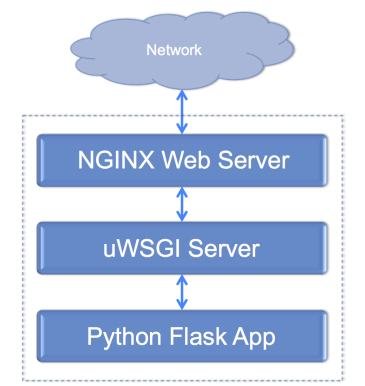
\includegraphics[width=0.6\textwidth]{images/server}
			\caption{Arquitectura del sistema}
	\end{figure}

	\subsection{Nginx}
		Nginx és...
	\subsection{uWSGI}
		asd
	\subsection{Flask}
		He decidit utilitzar Flask per desenvolupar l'aplicació web.

\section{Instal·lació del software}
	
	El sistema operatiu a utilitzar serà la versió lite de Raspbian, el sistema oficial de la fundació de Raspberry.
	Es pot baixar la imatge desde el web de raspberry i instal·lar a la targeta SD amb la comanda dd.\\

	\begin{bash}
	$ sudo dd bs=4M if=/home/joan/Downloads/raspbian.img
		of=/dev/mmcbk0
	\end{bash}

	Un cop tenim el sistema operatiu instal·lat, abans de començar a fer res, actualitzarem els paquets del sistema.\\

	\begin{bash}
	$ sudo apt-get update && sudo apt-get upgrade
	\end{bash}

	\subsubsection{Python}
	Instal·lar python, pip i dependencies del projecte\\
	\begin{bash}
	$ sudo apt-get install python3-pip python3-dev
	$ sudo apt-get install python3-numpy 
		python3-matplotlib
	\end{bash}

	\subsubsection{OpenCV}
	Instal·lar opencv Eines i biblioteques necessaries\\
	\begin{bash}
	$ sudo apt-get install cmake
	\end{bash}

	Imatges\\
	\begin{bash}
	$ sudo apt-get install libjpeg-dev libtiff5-dev
		libjasper-dev libpng12-dev
	\end{bash}
	Gtk\\
	\begin{bash}
	$ sudo apt-get install libgtk2.0-dev
	\end{bash}
	Optimitzacions\\
	\begin{bash}
	$ sudo apt-get install libatlas-base-dev gfortran
	\end{bash}

	Ens podem baixar OpenCV desde el repositori de github.\\
	\begin{bash}
	$ wget -O opencv.zip https://github.com/Itseez/
		opencv/archive/3.2.0.zip
	$ unzip opencv.zip
	\end{bash}

	Per poder utilitzar algorismes com SIFT i SURF també necessitarem descarregar OpenCV Contrib.\\
	\begin{bash}
	$ wget -O opencv_contrib.zip https://github.com/
		Itseez/opencv_contrib/archive/3.2.0.zip
	$ unzip opencv_contrib.zip
	\end{bash}

	Un cop obtinguts els arxius necessaris, podem preparar, compil·lar i instal·lar OpenCV al nostre sistema.\\
	\begin{bash}
	$ cd ~/opencv-3.2.0/
	$ mkdir build
	$ cd build
	$ cmake -D CMAKE_BUILD_TYPE=RELEASE \
		-D CMAKE_INSTALL_PREFIX=/usr/local \
		-D INSTALL_C_EXAMPLES=ON \
		-D INSTALL_PYTHON_EXAMPLES=ON \
		-D OPENCV_EXTRA_MODULES_PATH=
			~/opencv_contrib-3.2.0/modules \
		-D BUILD_EXAMPLES=ON ..

	$ make -j4
	$ sudo make install
	$ sudo ldconfig
	\end{bash}


	\subsubsection{Nginx}
	Per instal·lar el servidor web nomes cal utilitzar apt-get\\
	\begin{bash}
	$ sudo apt-get install nginx
	\end{bash}

	\subsubsection{Flask}
	Farem el mateix per instal·lar flask\\
	\begin{bash}
	$ sudo pip3 install flask
	\end{bash}

	\subsubsection{uWSGI}
	I ja nomes ens queda instal·lar uWSGI de la mateixa manera.\\
	\begin{bash}
	$ sudo pip3 install uwsgi
	\end{bash}

\section{Configuració}
	Ara que tenim tots els programes necessaris al servidor, ja podem configurar-lo perque s'executi la nostra aplicació web quan accedim
	a la IP del servidor.\\

	Creem un SGI Entry Point (wsgi.py)\\

	\begin{bash}
	$ nano ~/moras/wsgi.py
	\end{bash}

	\begin{python}
	from project import app

	if __name__ == "__main__":
		app.run()
	\end{python}

	També necessitem l'arxiu de configuració que utilitzarà uwsgi.\\

	\begin{bash}
	$ nano ~/moras/moras.ini
	\end{bash}

	\begin{txt}
	[uwsgi]
	module = wsgi:app

	master = true
	processes = 5

	socket = /tmp/moras.sock
	chmod-socket = 664
	vacuum = true

	die-on-term = true
	\end{txt}

	Amb això ja podriem executar uwsgi sense problemes, pero volem que el servei s'executi de manera automàtica quan iniciem el sistema.
	Per aconseguir això, afegirem una linia al fitxer rc.local que s'encarregui d'executar l'arxiu .ini creat anteriorment.\\

	\begin{bash}
	$ sudo nano /etc/rc.local
	\end{bash}

	\begin{txt}
	[...]

	/usr/local/bin/uwsgi --ini /home/pi/moras/moras.ini
		--uid www-data --gid www-data
		--daemonize /var/log/uwsgi.log

	exit 0
	\end{txt}

	Per tal que Nginx redirigeixi les peticions al servidor uWSGI, hem de crear un nou lloc a /etc/nginx/sites-available.\\
	\begin{bash}
	$ sudo nano /etc/nginx/sites-available/moras
	\end{bash}

	\begin{txt}
	server {
		listen 80;
		server_name localhost;

		location / {
			include uwsgi_params;
			uwsgi_pass unix:/tmp/moras.sock;
		}
	}
	\end{txt}

	Finalment, nomes caldrà activar el lloc web creant un soft link a sites-enabled i reiniciar el servidor Nginx
	per aplicar la nova configuració.\\
	\begin{bash}
	$ sudo ln -s /etc/nginx/sites-available/moras
		/etc/nginx/sites-enabled
	$ sudo systemctl restart nginx
	\end{bash}
